\documentclass[11pt]{article}
\usepackage{svg}
\usepackage{graphicx}

\pagestyle{plain}
\title{Rapport 2 : Décomposition LU et moindres carrés}
\author{Loïc Jabiro KAYITAKIRE}
\date{NOMA : 53272100}

\begin{document}
\maketitle

\section*{Question 1}

\subsection*{Définition}
Le conditionnement est un concept qui permet de mesurer la sensibilité d'un problème de calcul numérique par rapport à une perturbation. 
Il est mesuré grâce au nombre de conditionnement $ \kappa $ qui se calcule comme suit :
$$ \kappa(x) = \lim_{\delta \to 0}   \sup_{||\delta x|| \leq \delta}   \frac{\frac{||\delta x||}{||x||}}{\frac{||\delta A||}{||A||}} $$

\subsection*{Conditionnement par rapport à A}

Le problème de base est : $A^T A x = A^T B$
\\
On pose $A^T A = A'$ et $A^T B = B'$
\\
On suppose une perturbation $ \delta A' $ sur A'. On a alors le problème perturbé suivant : 
$$ (A' + \delta A') (x + \delta x) = B' $$
$$ A'x + A'\delta x + \delta A'x + \delta A' \delta x = B' $$
$ A'x = B'$ et $ \delta A' \delta x$ est négligeable par rapport au reste. On a alors :
$$ A'\delta x + \delta A' x = 0 $$
Ce qui donne ensuite :
$$ \delta x = -A'^{-1} \delta A' x $$
On a alors :
$$ ||\delta x|| = ||-A'^{-1} \delta A' x|| \leq ||A'^{-1}|| ||\delta A'|| ||x|| $$
Et donc :
$$ \frac{||\delta x||}{||x||} \leq ||A'||||A'^{-1}|| \frac{||\delta A'||}{||A'||} $$

Ainsi, $ \kappa(A^T A) = ||A^T A||||(A^T A)^{-1}|| $ 

En suivant un raisonnement similaire pour une perturbation sur B, on obtient :
$$ \kappa(A^T B) = ||A^T B||||(A^T A)^{-1}|| $$

\section*{Question 2}

La complexité est $O(n^3)$ pour la décomposition LU. L'algorithme n'est pas parallélisable car les calculs dépendent des résultats précédents.
%Add image
\begin{figure}[h]
\centering
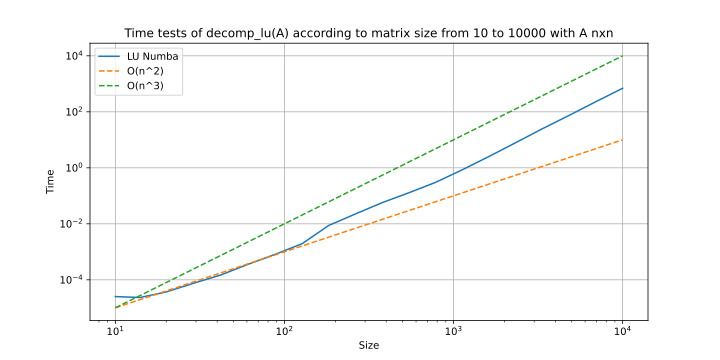
\includegraphics[width=0.5\textwidth]{images/lu_time_tests.pdf}
\caption{Temps d'exécution de la décomposition LU en fonction de la taille de la matrice}
\end{figure}

\section*{Question 3}

\section*{Question 4}
Pour des équations normales de la forme $A^T A x = A^T B$, on a que $A^T A$ est symétrique et définie positive. 
On peut donc effectuer l'élimination gaussienne sur les deux côtés de la diagonale de la matrice, étant donné que la matrice est symétrique.
On obtient alors la décomposition de Cholesky dont la complexité est $O(n^3/3)$. On effectue ainsi deux fois moins d'opérations.

\begin{figure}[h]
\centering
\includegraphics[width=0.5\textwidth]{images/lu_cholesky_time_tests.pdf}
\caption{Temps d'exécution de la décomposition LU et de Cholesky en fonction de la taille de la matrice}
\end{figure}

\begin{figure}[h]
\centering
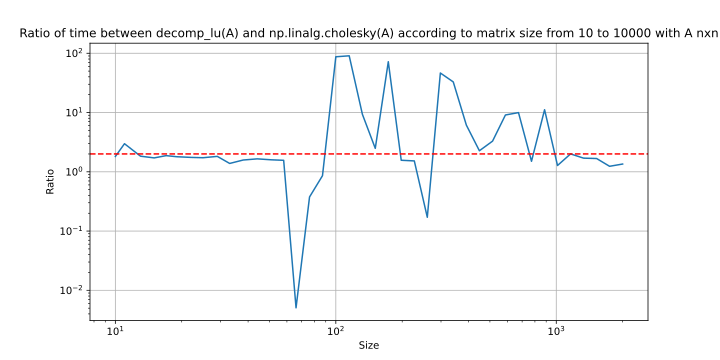
\includegraphics[width=0.5\textwidth]{images/lu_cholesky_ratio.pdf}
\caption{Rapport des temps d'exécution de la décomposition LU et de Cholesky en fonction de la taille de la matrice}

\end{figure}



\end{document}